\begin{enumerate}
    \item Определение. Естественность и полезность

    \begin{definition}
    Пусть $E$~--- нормированное пространство. Говорим, что последовательность элементов $x_n$ \textit{слабо сходится} к $x$, обозн. ($x_n \weakconv x$), если \[\forall f \in E^*\; f(x_n) \to f(x).\]
    \end{definition}

    \item Корректность определения. Хотим показать единственность предела.

    Предположим, что $x_n \weakconv x'$ и $x_n \weakconv x''$. По определению 

    \[ \forall f \in E^* \; f(x_n) \to f(x'), \; f(x_n) \to f(x'')  \quad \Rightarrow \quad \forall f \in E^* \; f(x') = f(x'')\]

    А по следствию~\nameref{hbcorollary3} из теоремы Хана-Банаха верно, что \(x' = x''\).

    \item Сравнение слабой сходимости и сходимости по норме
    \begin{itemize}
        \item $\dim E$~--- любая.
        \[\|x_n - x\| \to 0 \implies x_n \weakconv x.\]
        \begin{proof}
            \(|f(x_n)-f(x)|=|f(x_n-x)| \leqslant \|f\| \cdot \|x_n - x\| \to 0\)
        \end{proof}
        \item $\dim E < \infty$
        \[\|x_n - x\| \to 0 \Leftarrow x_n \weakconv x.\]
        \begin{proof}
            Рассмотрим функционалы
            \begin{multline*}
            f_k \in E^*:\; f_k x = x^k\text{ ($k$-ая координата)};\\
                x_n \weakconv x \implies \forall k \in \overline{1, \dim E}\;\; f_k (x_n) \to f(x) \implies x_n^k \to x^k.
            \end{multline*}
            Из покоординатной сходимости в конечномерном пространстве следует сходимость по норме.
        \end{proof}
        \item $\dim E = \infty$
        \[\|x_n - x\| \to 0 \not\Leftarrow x_n \weakconv x.\]

        \begin{counterexample} $H = l_2(\R),\: e^n = (0, \ldots, 0, 1, 0 \ldots)$. Понятно, что сходимости по норме нет. Однако, если рассмотреть определение и перейти к скалярному произведению:
        \[ \angles{e^n, y} = y_n \to 0 = \angles{0, y}.\]
        Причём \(y_n\) стремится к нулю как член сходящегося ряда. Откуда получаем, что $e^n \weakconv 0$.
        \end{counterexample}
    \end{itemize}

    \item Слабая сходимость в гильбертовом пространстве

    Пусть $H$ ~--- гильбертово пространство. По теореме~\nameref{Riss-Freshe} $f(x)=\angles{x, y},\; y \in H$. Тогда $f(x_n) \to f(x) \Leftrightarrow \angles{x_n, y} \to \angles{ x, y }$.

    Можно ли придумать норму, которая порождает эту сходимость? \textbf{Нет, нельзя и это нетривиальный факт}.
    \item В гильбертовом пространстве $\| x_n - x \| \to 0 \implies x_n \weakconv x.$\\
    Можно ли к слабой сходимости добавить условие, чтобы обе части были равносильны?
    В гильбертовом пространстве можно, достаточно чтобы $\|x_n\| \to \|x\|$. (Из дз \S 10 №9).

    \item \textbf{Изометрия} $E$ и $E^{**}$
    
    Пусть $\pi: E \to E^{**}$ такое, что $\pi x = F_x \in E^{**}, \; F_x(f) = f(x)$, где $f\in E^*$
    \begin{figure}[H]
            \centering
            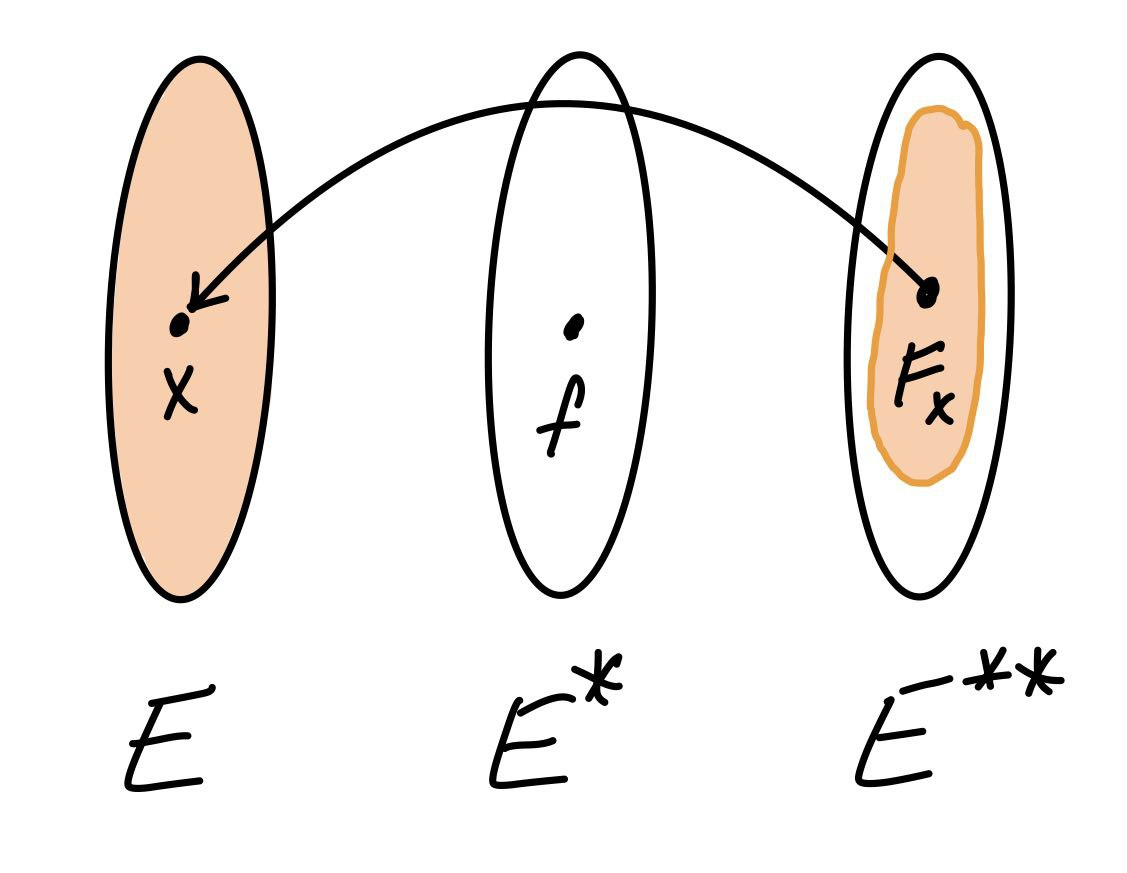
\includegraphics[width=0.35\textwidth]{images/isometry.jpg}
    \end{figure}
    В силу следствия~\nameref{hbcorollary4} из теоремы Хана-Банаха отображение $\pi$ -- изометрия:

    \[ \| F_x \| \stackrel{def} {=} \sup_{\|f\|=1} |F_x(f)|=\sup_{\| f \| = 1} |f(x)| \stackrel{\text{сл. 4}}{=}||x|| \]

    \begin{note}
    \[x_n \weakconv x \; \stackrel{def} {\Longleftrightarrow} \; \forall f \ f(x_n) \to f(x) \; \Longleftrightarrow \; \forall f \ F_{x_n}(f) \to F_x(f) \]
    Это означает поточечную сходимость $F_{x_n}$ к $F_x$.
    \end{note}
    
    \item Вспоминаем следствие теоремы~\nameref{Banach-Steingaus}:~\nameref{bshetengcorollary}.
    Сейчас у нас операторы $F_x\!: E^* \to \K$. Помним, что так как $\K$~--- полное, то $E^*=\mathcal{L}(E, \K)$~--- полное.

    \begin{theorem}[Критерий слабой сходимости]\label{criteria_weak_to}
        Пусть $E$~--- ЛНП. Тогда последовательность $x_n \in E,\; x_n \weakconv x$ тогда и только тогда когда выполнено:\\
        \[\begin{cases}
        \text{1) последовательность $\{\|x_n\|\}$~--- ограничена}\\
        \text{2) $\forall s \in S \subset E^*\!: \overline{[S]} = E^*,\;\; s(x_n) \to s(x )$}\\
        \end{cases}\]
    \end{theorem}

    \begin{proof}
        Очевидным образом вытекает из изометрии и упомянутого следствия теоремы Банаха-Штейнгауза.
    \end{proof}

\end{enumerate}

